\newpage
\section{Appendix}
\usepackage{float}
\subsection{Control Plots}
\label{sect:Appendix}
We performed some checks to justify our analysis cuts. Our cuts were optimised based on maximization of the statistical significance. We studied our main cuts in this analysis.
In Figure \ref{fig:MT2diffVSPT} we show the \mttwo distribution for QCD for different intervals of VSPT. The different distributions 
are normalized to the same area. The variable is plotted for QCD events that
pass the cuts described above. From Figure \ref{fig:MT2diffVSPT}, we see that for
large values of VSPT, the \mttwo distribution is distorted and deviates from the distribution with
$0 <$ VSPT $<20$, i.e. small VSPT. Since the distortion becomes significant for VSPT $> 70$ GeV, we
cut away events above this value. 
\begin{figure}[!Hhtb]
\begin{center}
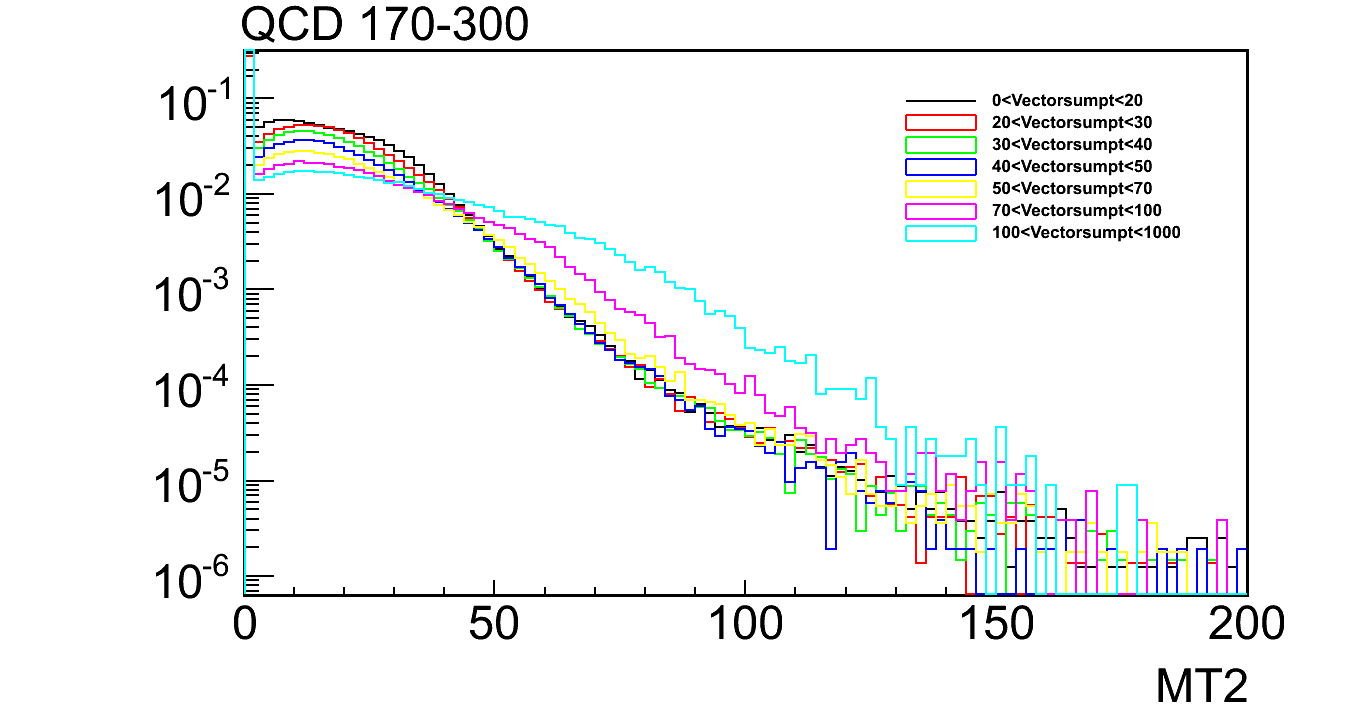
\includegraphics[angle=00,width=0.5\textwidth]{figs/MT2-diffVSPT-QCD170-300.png}\\
%	\mbox{\small{(1)} \\
\end{center}
\caption{Disrtibution of \mttwo in different VSPT ranges for one QCD sample}
\label{fig:MT2diffVSPT}
\end{figure}
  
We looked at the distributions of different variables before and after applying VSPT $<70$ when the other cuts 
except $\mttwo > 125 $ were relaxed. As it is obvious from Figures \ref{fig:MT2VSPT}-\ref{fig:VSPTVSPT}, by applying VSPT $<70$ we have better agreement 
between data and MC,

\begin{figure}[!Hhtb] %[!Hhtb]
\begin{center}$
\begin{array}{cc} 
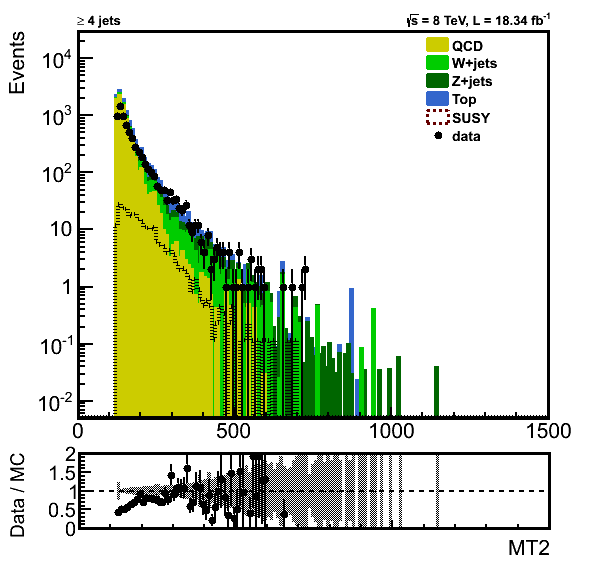
\includegraphics[angle=00,width=0.5\textwidth]{figs/MT2-beforeVSPT-NocutExMT2.png}&
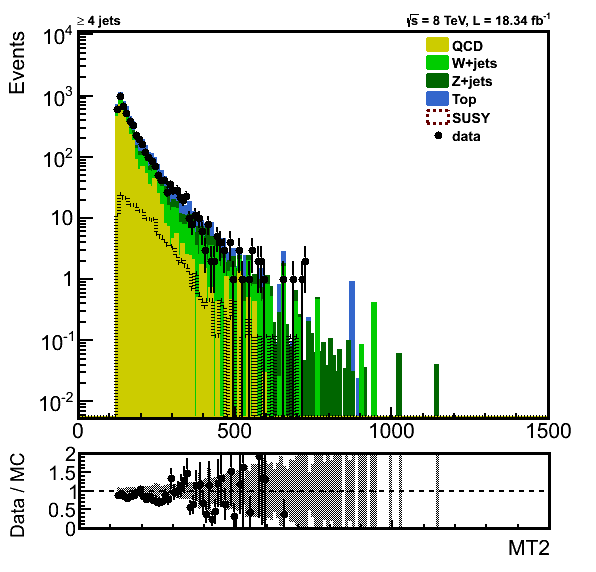
\includegraphics[angle=00,width=0.5\textwidth]{figs/MT2-afterVSPT-NocutExMT2.png}\\
  \mbox{\small{(a)}} & \mbox{\small{(b)}} \\
\end{array}$
\end{center}
\caption{Distribution of \mttwo before(a) and after(b) applying VSPT $< 70$}
\label{fig:MT2VSPT}
\end{figure}

\begin{figure}[!Hhtb]
\begin{center}$
\begin{array}{cc} 
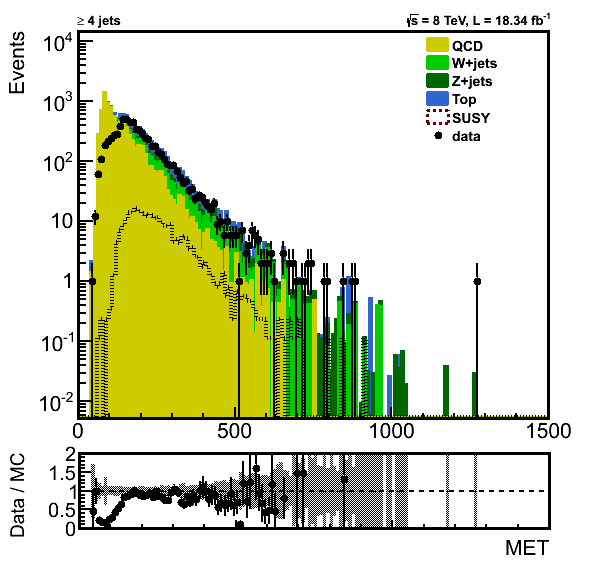
\includegraphics[angle=00,width=0.5\textwidth]{figs/MET-beforeVSPT-NocutExMT2.png}&
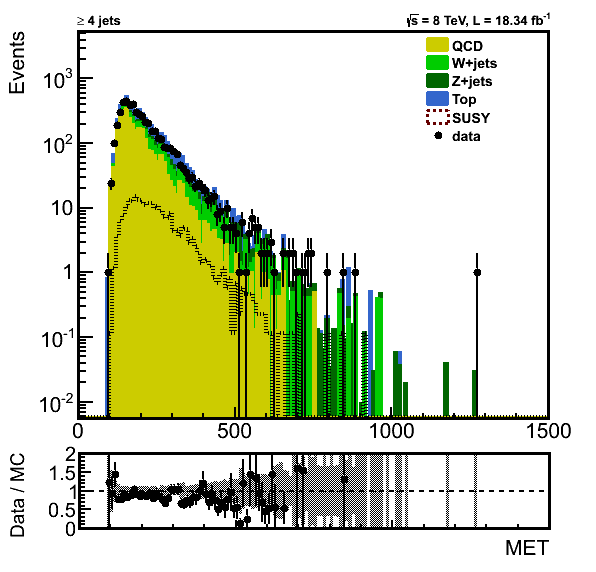
\includegraphics[angle=00,width=0.5\textwidth]{figs/MET-afterVSPT-NocutExMT2.png}\\
	\mbox{\small{(a)}} & \mbox{\small{(b)}} \\
\end{array}$
\end{center}
\caption{Distribution of \met before(a) and after(b) applying VSPT $< 70$}
\label{fig:METVSPT}
\end{figure}

\begin{figure}[!Hhtb]
\begin{center}$
\begin{array}{cc} 
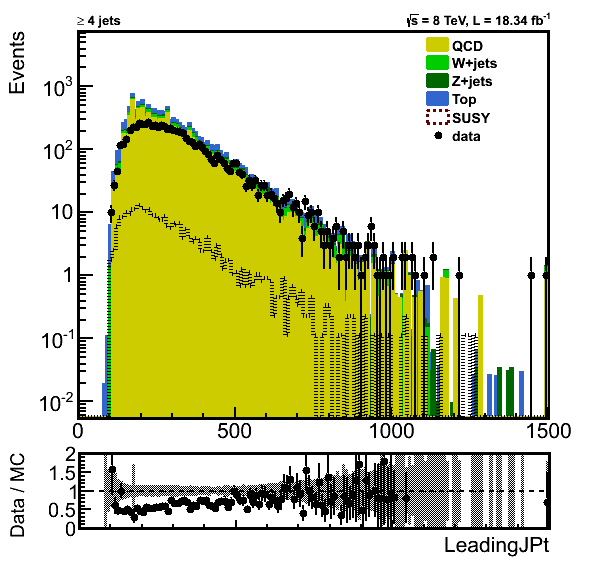
\includegraphics[angle=00,width=0.5\textwidth]{figs/LeadJPt-beforeVSPT-NocutExMT2.png}&
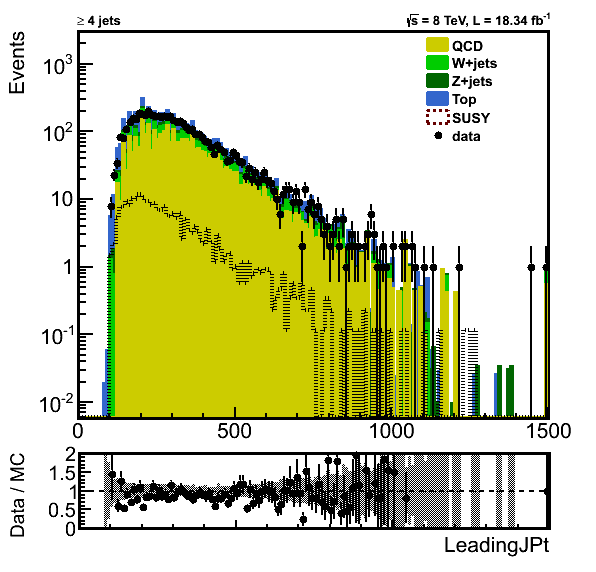
\includegraphics[angle=00,width=0.5\textwidth]{figs/LeadJPt-afterVSPT-NocutExMT2.png}\\
	\mbox{\small{(a)}} & \mbox{\small{(b)}} \\
\end{array}$
\end{center}
\caption{Distribution of Leading Jet $P_{t}$ before(a) and after(b) applying VSPT $< 70$}
\label{fig:LeadJetPtVSPT}
\end{figure}

\begin{figure}[!Hhtb]
\begin{center}$
\begin{array}{cc} 
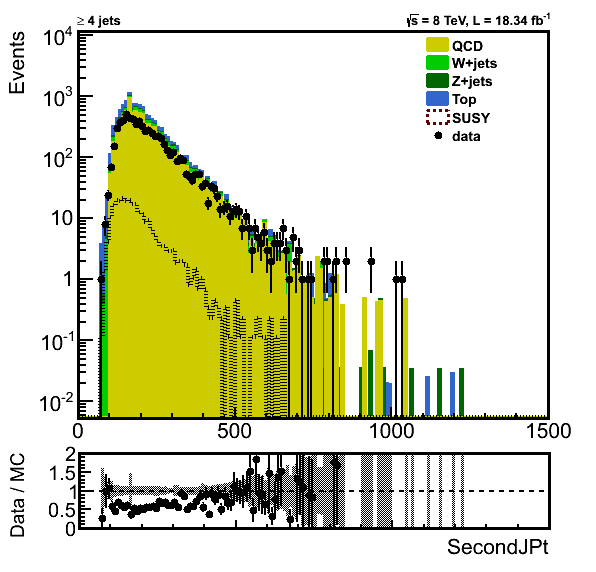
\includegraphics[angle=00,width=0.5\textwidth]{figs/SecJPt-beforeVSPT-NocutExMT2.png}&
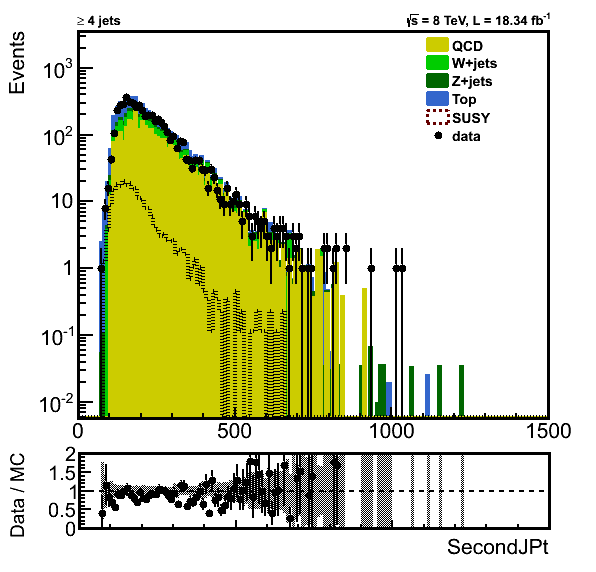
\includegraphics[angle=00,width=0.5\textwidth]{figs/SecJPt-afterVSPT-NocutExMT2.png}\\
	\mbox{\small{(a)}} & \mbox{\small{(b)}} \\
\end{array}$
\end{center}
\caption{Distribution of Second Jet $P_{t}$ before(a) and after(b) applying VSPT $< 70$}
\label{fig:SecJetPtVSPT}
\end{figure}

\begin{figure}[!Hhtb]
\begin{center}$
\begin{array}{cc} 
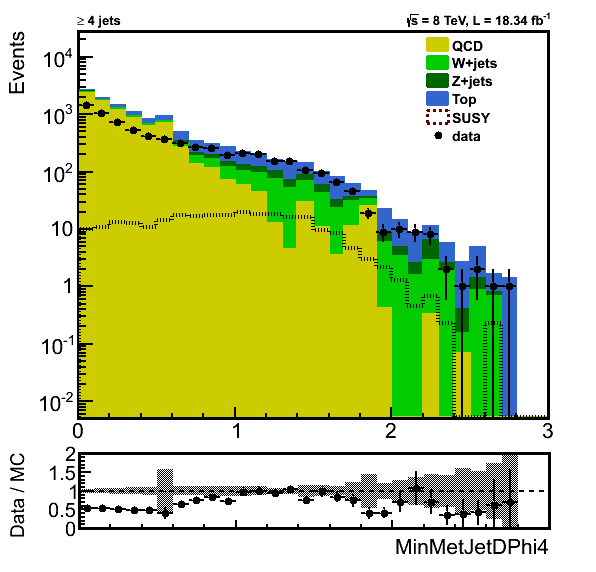
\includegraphics[angle=00,width=0.5\textwidth]{figs/MinMETJDPhi4-beforeVSPT-NocutExMT2.png}&
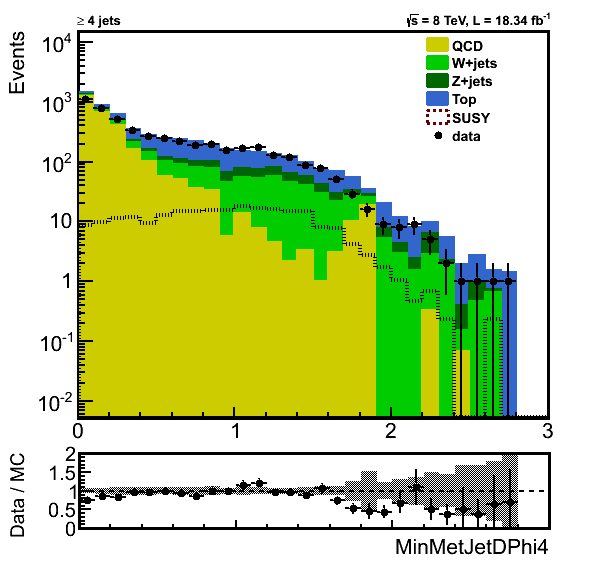
\includegraphics[angle=00,width=0.5\textwidth]{figs/MinMETJDPhi4-afterVSPT-NocutExMT2.png}\\
	\mbox{\small{(a)}} & \mbox{\small{(b)}} \\
\end{array}$
\end{center}
\caption{Distribution of \mindphifour before(a) and after(b) applying VSPT $< 70$}
\label{fig:MinDPhiVSPT}
\end{figure}

\begin{figure}[!Hhtb]
\begin{center}$
\begin{array}{cc} 
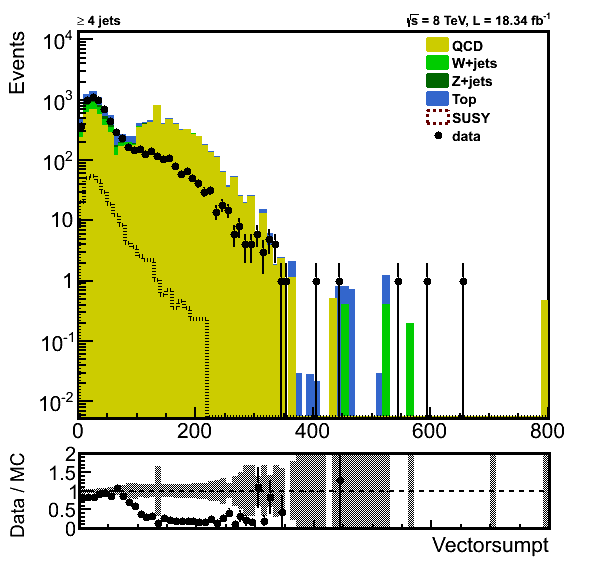
\includegraphics[angle=00,width=0.5\textwidth]{figs/VSPT-beforeVSPT-NocutExMT2.png}&
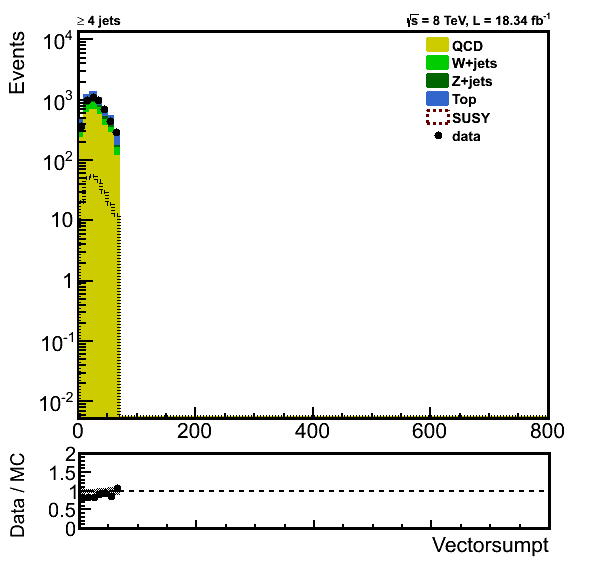
\includegraphics[angle=00,width=0.5\textwidth]{figs/VSPT-afterVSPT-NocutExMT2.png}\\
	\mbox{\small{(a)}} & \mbox{\small{(b)}} \\
\end{array}$
\end{center}
\caption{Distribution of VSPT before(a) and after(b) applying VSPT $< 70$}
\label{fig:VSPTVSPT}
\end{figure}


To justify the cut on \mindphifour which is $\mindphifour > 0.3$, like VSPT, We looked at the distributions of different variables before and after applying $\mindphifour > 0.3$ when the other cuts 
except $\mttwo > 125 $ were relaxed. As it is obvious from figures \ref{fig:MT2MinDPhi}-\ref{fig:VSPTMinDPhi}, 
by applying $\mindphifour > 0.3$ we have a better agreement 
between data and MC, 

\begin{figure}[!Hhtb]
\begin{center}$
\begin{array}{cc} 
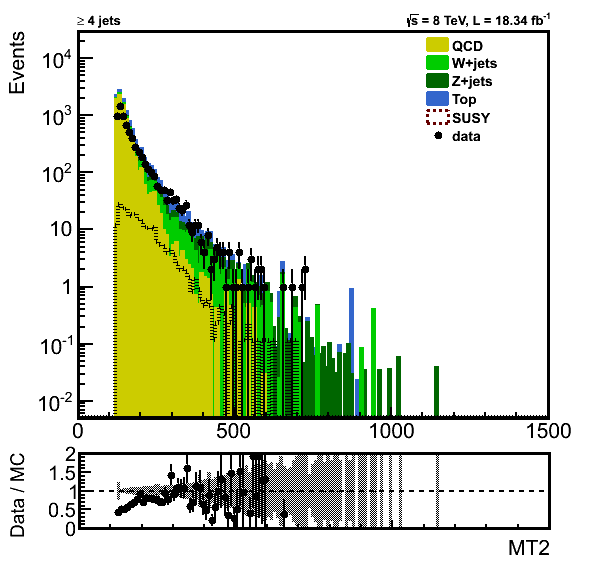
\includegraphics[angle=00,width=0.5\textwidth]{figs/MT2-beforeVSPT-NocutExMT2.png}&
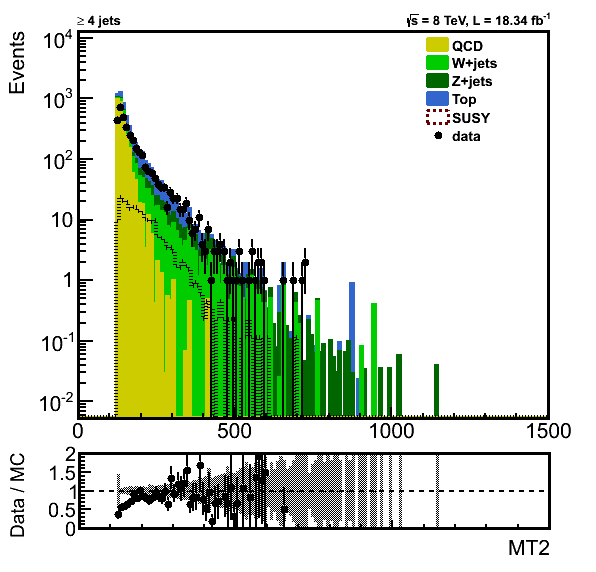
\includegraphics[angle=00,width=0.5\textwidth]{figs/MT2-afteDPhi-NocutExMT2.png}\\
	\mbox{\small{(a)}} & \mbox{\small{(b)}} \\
\end{array}$
\end{center}
\caption{Distribution of \mttwo before(a) and after(b) applying $\mindphifour > 0.3$}
\label{fig:MT2MinDPhi}
\end{figure}

\begin{figure}[!Hhtb]
\begin{center}$
\begin{array}{cc} 
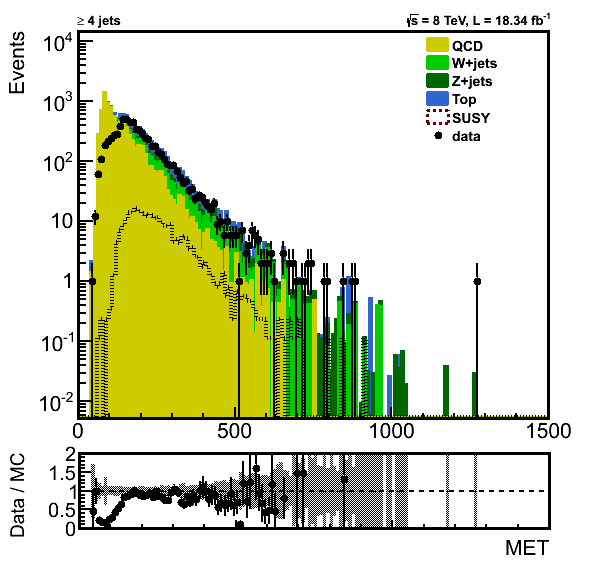
\includegraphics[angle=00,width=0.5\textwidth]{figs/MET-beforeVSPT-NocutExMT2.png}&
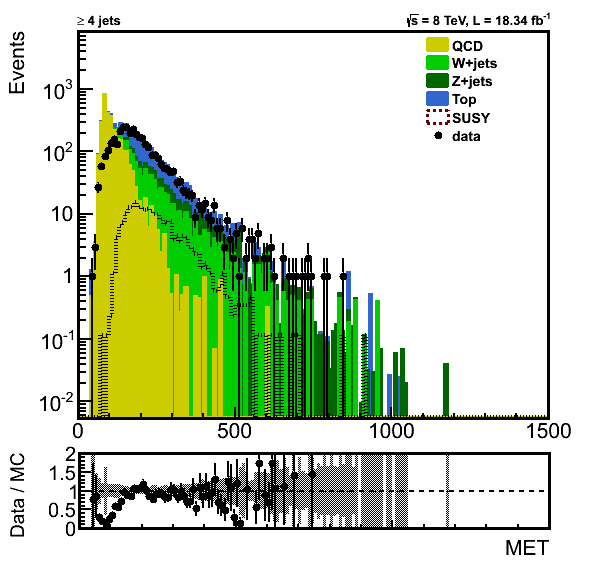
\includegraphics[angle=00,width=0.5\textwidth]{figs/MET-afteDPhi-NocutExMT2.png}\\
	\mbox{\small{(a)}} & \mbox{\small{(b)}} \\
\end{array}$
\end{center}
\caption{Distribution of \met before(a) and after(b) applying $\mindphifour > 0.3$}
\label{fig:METMinDPhi}
\end{figure}

\begin{figure}[!Hhtb]
\begin{center}$
\begin{array}{cc} 
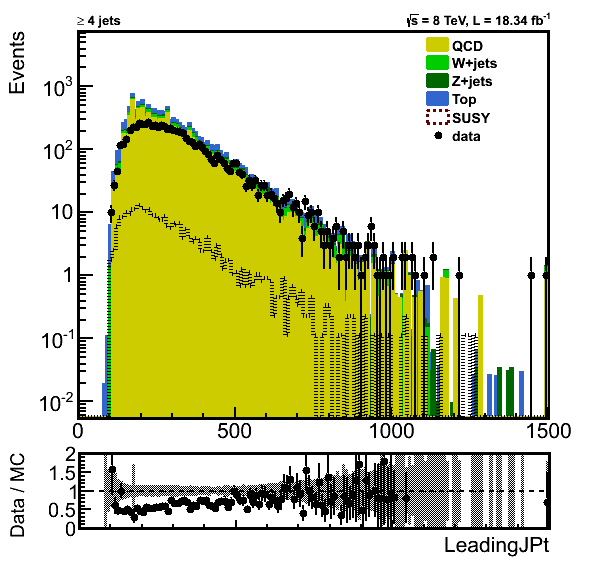
\includegraphics[angle=00,width=0.5\textwidth]{figs/LeadJPt-beforeVSPT-NocutExMT2.png}&
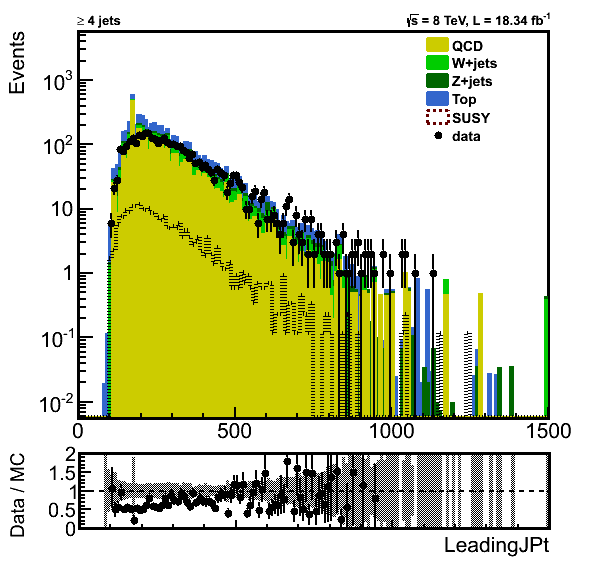
\includegraphics[angle=00,width=0.5\textwidth]{figs/LeadJPt-afterDPhi-NocutExMT2.png}\\
	\mbox{\small{(a)}} & \mbox{\small{(b)}} \\
\end{array}$
\end{center}
\caption{Distribution of Leading Jet $P_{T}$ before(a) and after(b) applying $\mindphifour > 0.3$}
\label{fig:LeadJetPtMinDPhi}
\end{figure}

\begin{figure}[!Hhtb]
\begin{center}$
\begin{array}{cc} 
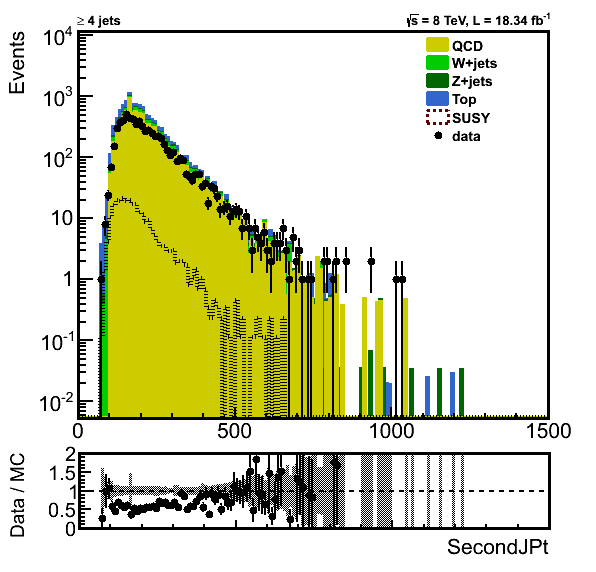
\includegraphics[angle=00,width=0.5\textwidth]{figs/SecJPt-beforeVSPT-NocutExMT2.png}&
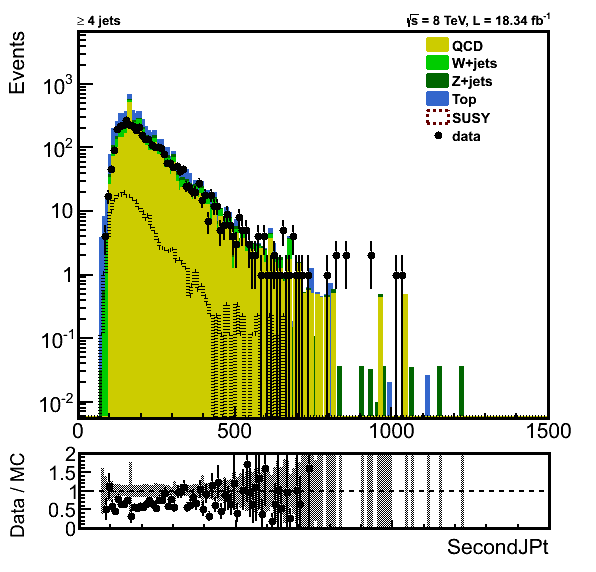
\includegraphics[angle=00,width=0.5\textwidth]{figs/SecJPt-afterDPhi-NocutExMT2.png}\\
%	\mbox{\small{(a)}} & \mbox{\small{(b)}} \\
\end{array}$
\end{center}
\caption{Distribution of Second Jet $P_{T}$ before(a) and after(b) applying $\mindphifour > 0.3$}
\label{fig:SecJetPtMinDPhi}
\end{figure}

\begin{figure}[!Hhtb]
\begin{center}$
\begin{array}{cc} 
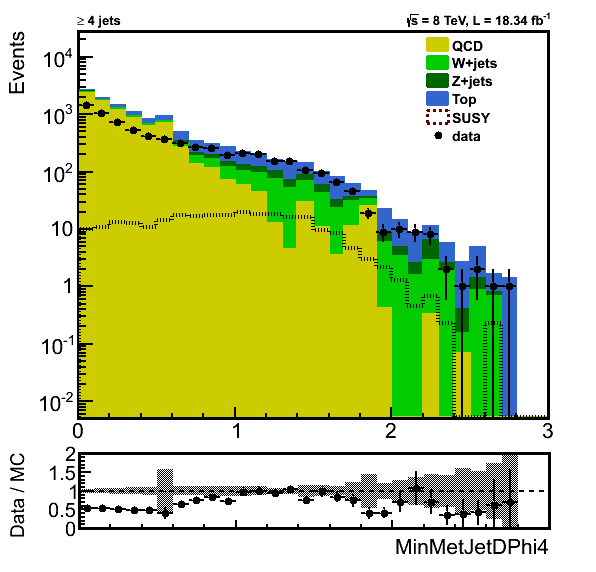
\includegraphics[angle=00,width=0.5\textwidth]{figs/MinMETJDPhi4-beforeVSPT-NocutExMT2.png}&
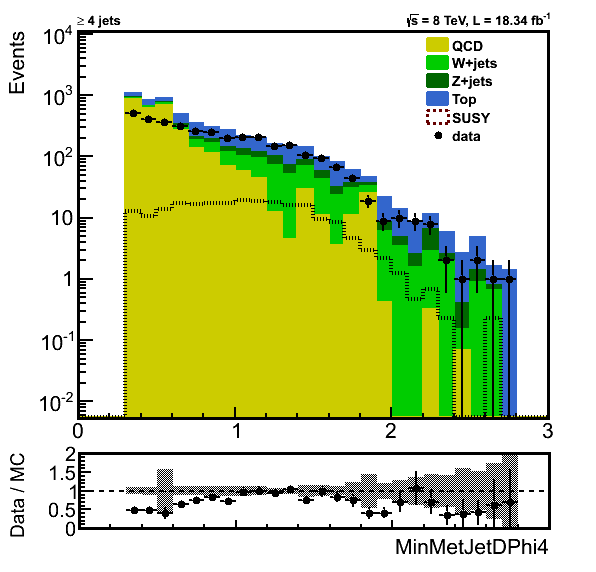
\includegraphics[angle=00,width=0.5\textwidth]{figs/MinMETJDPhi4-afterDPhi-NocutExMT2.png}\\
	\mbox{\small{(a)}} & \mbox{\small{(b)}} \\
\end{array}$
\end{center}
\caption{Distribution of \mindphifour before(a) and after(b) applying $\mindphifour > 0.3$}
\label{fig:MinDPhiMinDPhi}
\end{figure}

\begin{figure}[!Hhtb]
\begin{center}$
\begin{array}{cc} 
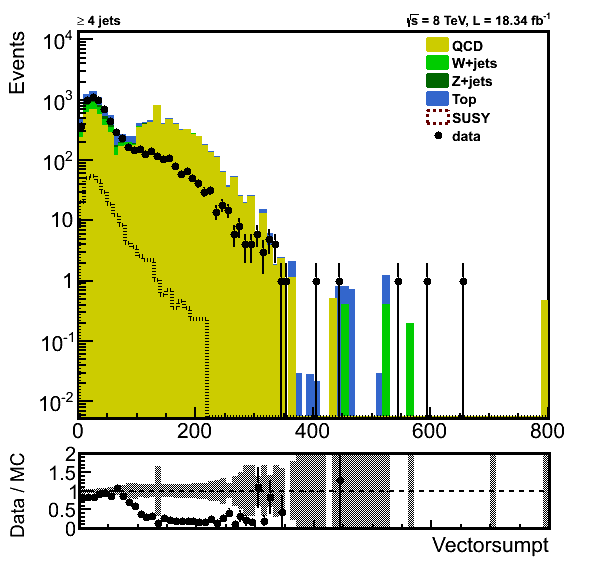
\includegraphics[angle=00,width=0.5\textwidth]{figs/VSPT-beforeVSPT-NocutExMT2.png}&
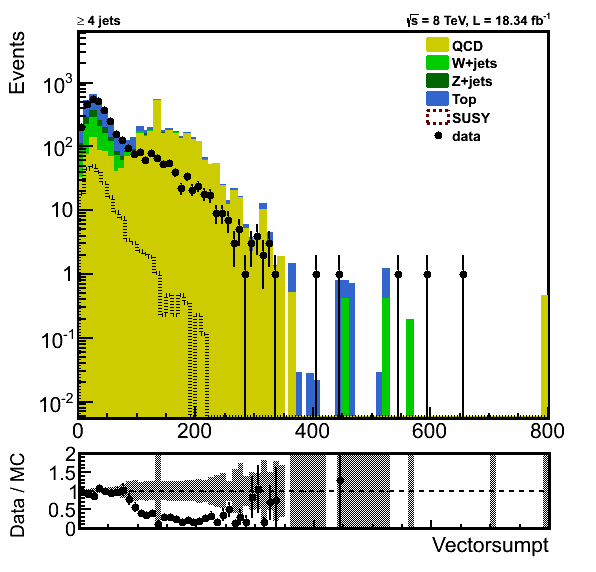
\includegraphics[angle=00,width=0.5\textwidth]{figs/VSPT-afterDPhi-NocutExMT2.png}\\
	\mbox{\small{(a)}} & \mbox{\small{(b)}} \\
\end{array}$
\end{center}
\caption{Distribution of VSPT before(a) and after(b) applying $\mindphifour > 0.3$}
\label{fig:VSPTMinDPhi}
\end{figure}

%
%We applied Jet-Met smearing on MC samples and then plotted the distributions of \met and \mttwo. As it is seen below
%there is an excellent agreement between Data and MC in both cases.

%\begin{figure}[!Hhtb]
%\begin{center}$
%\begin{array}{cc} 
%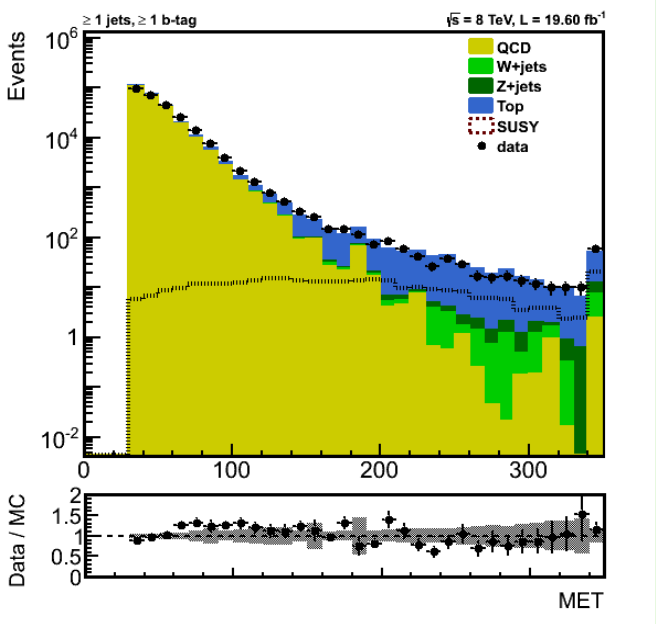
\includegraphics[angle=00,width=0.5\textwidth]{figs/MET-before-JMS.png}&
%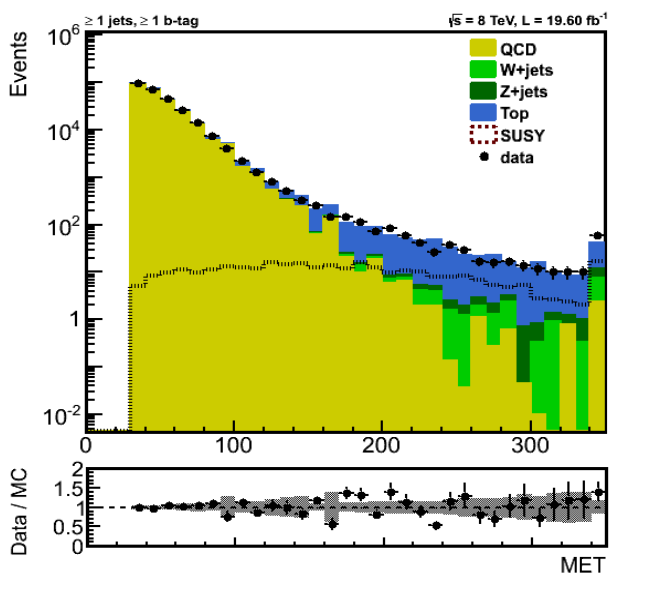
\includegraphics[angle=00,width=0.5\textwidth]{figs/MET-after-JMS.png}\\
%	\mbox{\small{(a)}} & \mbox{\small{(b)}} \\
%\end{array}$
%\end{center}
%\caption{Distribution of \met before(a) and after(b) applying Jet-MET smearing}
%\label{fig:METJetMETSmear}
%\end{figure}


%\begin{figure}[!Hhtb]
%\begin{center}$
%\begin{array}{cc} 
%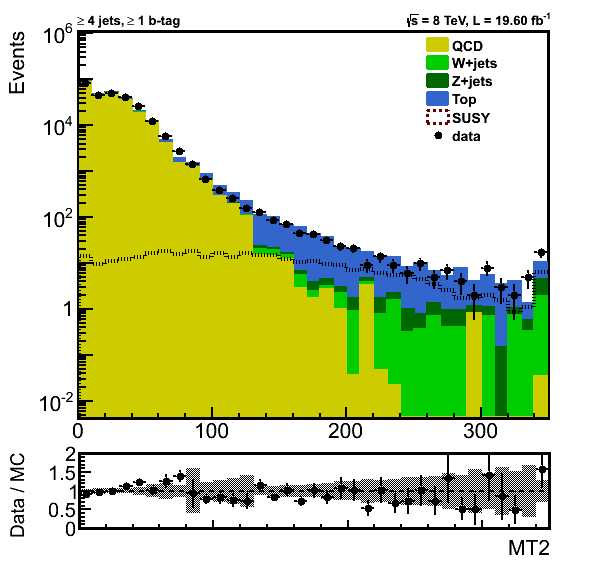
\includegraphics[angle=00,width=0.5\textwidth]{figs/MT2-before-JMS.png}&
%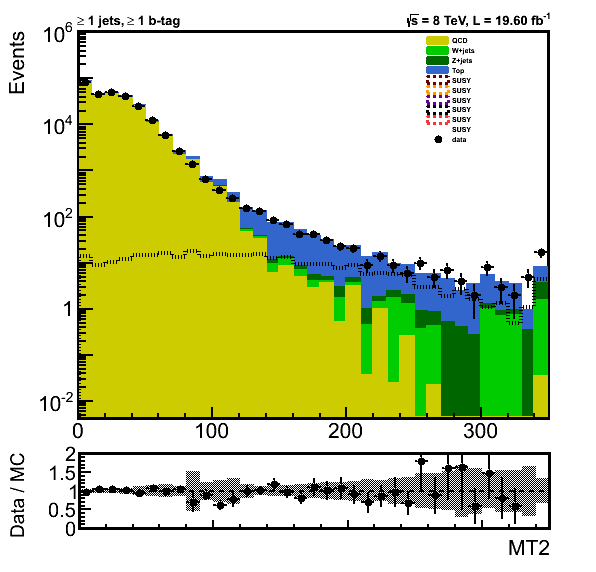
\includegraphics[angle=00,width=0.5\textwidth]{figs/MT2-after-JMS.png}\\
%	\mbox{\small{(a)}} & \mbox{\small{(b)}} \\
%\end{array}$
%\end{center}
%\caption{Distribution of \mttwo before(a) and after(b) applying Jet-MET smearing}
%\label{fig:MT2JetMETSmear}
%\end{figure}

We applied pile-up reweighting and b-tagging scale factor and to see that these 
effects are under control, we looked at the number of CSVT b jets,


\begin{figure}[!Hhtb]
\begin{center}
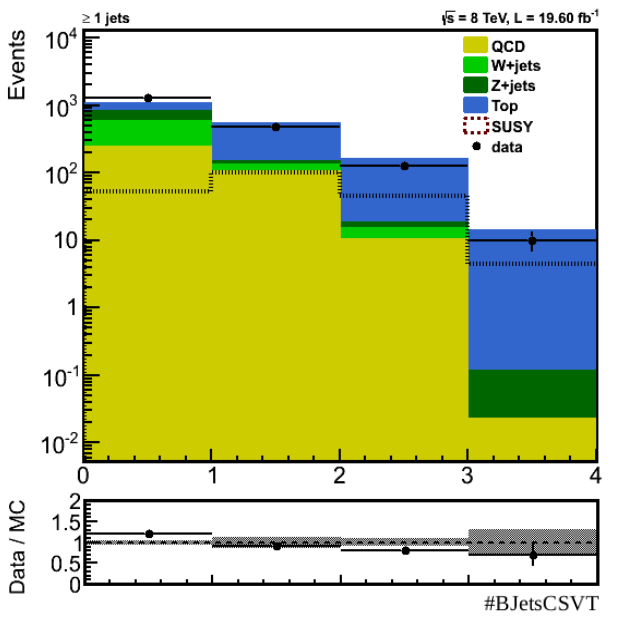
\includegraphics[angle=00,width=0.5\textwidth]{figs/NB-noSF-noPU-noJMS.png}
\caption{(a).no b-tagging scale factor, no pile-up re-weighting} \\
\end{center}
\begin{center}$
\begin{array}{cc}
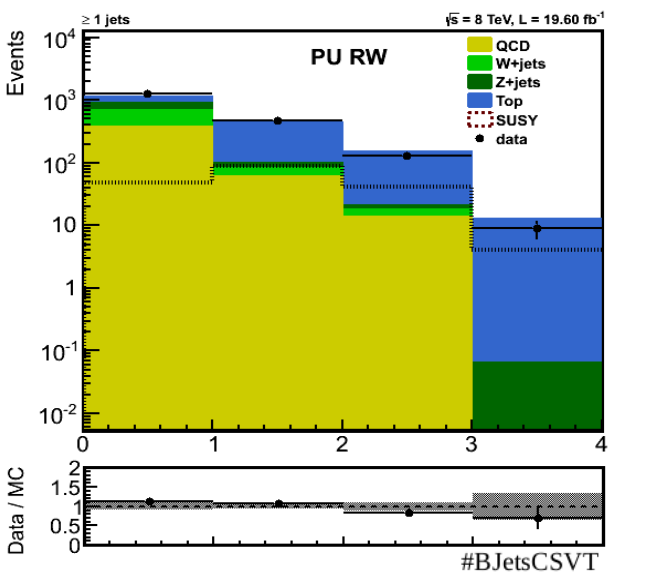
\includegraphics[angle=00,width=0.5\textwidth]{figs/NB-noSF-PU-JMS.png}&
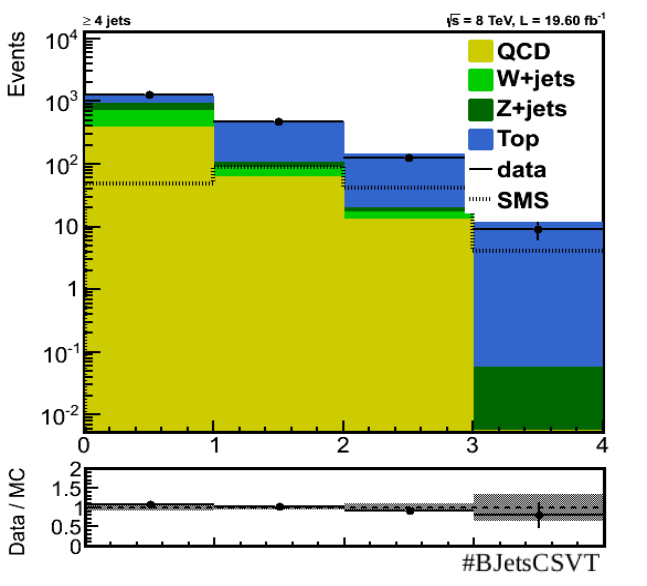
\includegraphics[angle=00,width=0.5\textwidth]{figs/NB-SF-PU-JMS.png}\\
	\mbox{\small{(b). no b-tagging scale factor, pile-up re-weighted}} & \mbox{\small{(c). b-tagging scale factor applied,pile-up reweighted}} \\
\end{array}$
\end{center}
\caption{Effects of applying pile-up reweighting and b-tagging scale factor on distribution of number of CSVT b jets}
\label{fig:NBCSVTPileUpJetMETSmearSF}
\end{figure}

%It was also checked the correlation of between variables \mttwo and \met for different samples. It is seen that 
%there is a correlation betwwn these two variables and events having hight \met sit in the high \mttwo region.  
%\begin{figure}[!Hhtb]
%\begin{center}$
%\begin{array}{ccc} 
%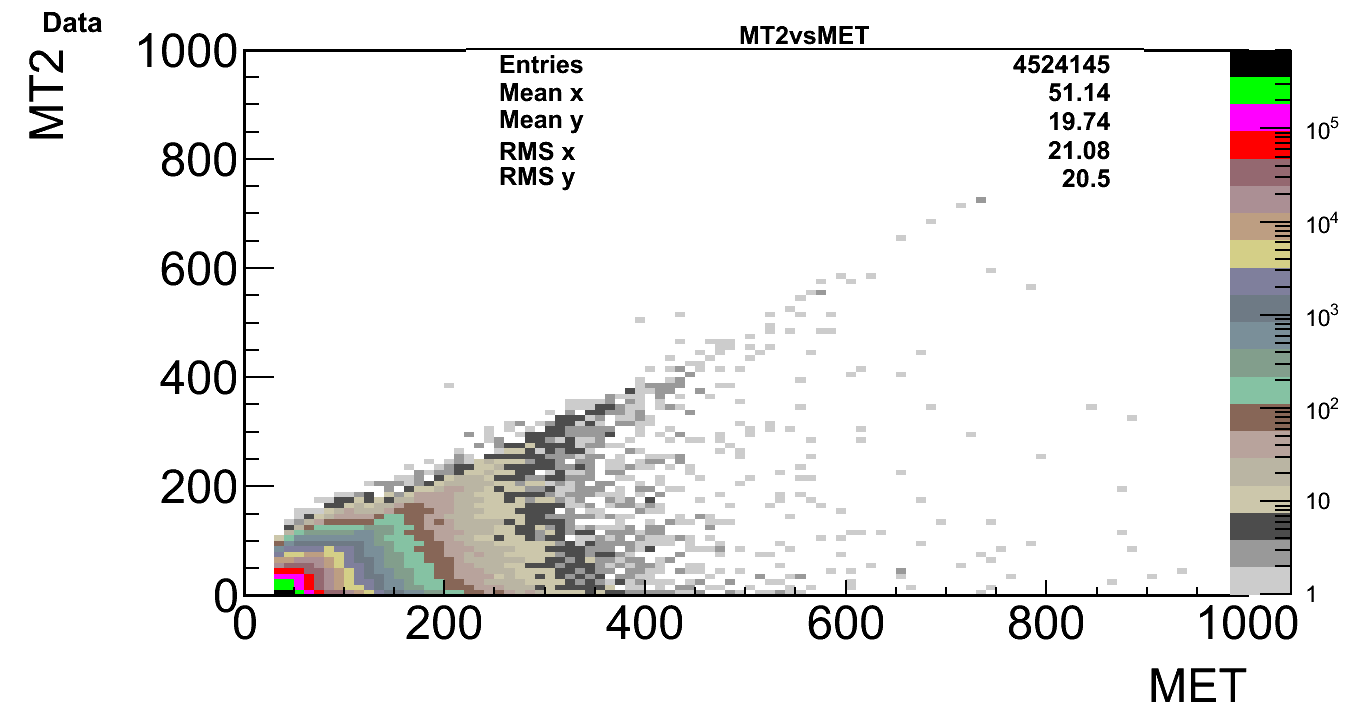
\includegraphics[angle=00,width=0.5\textwidth]{figs/MT2-MET-before-AllCuts--Data.png}&
%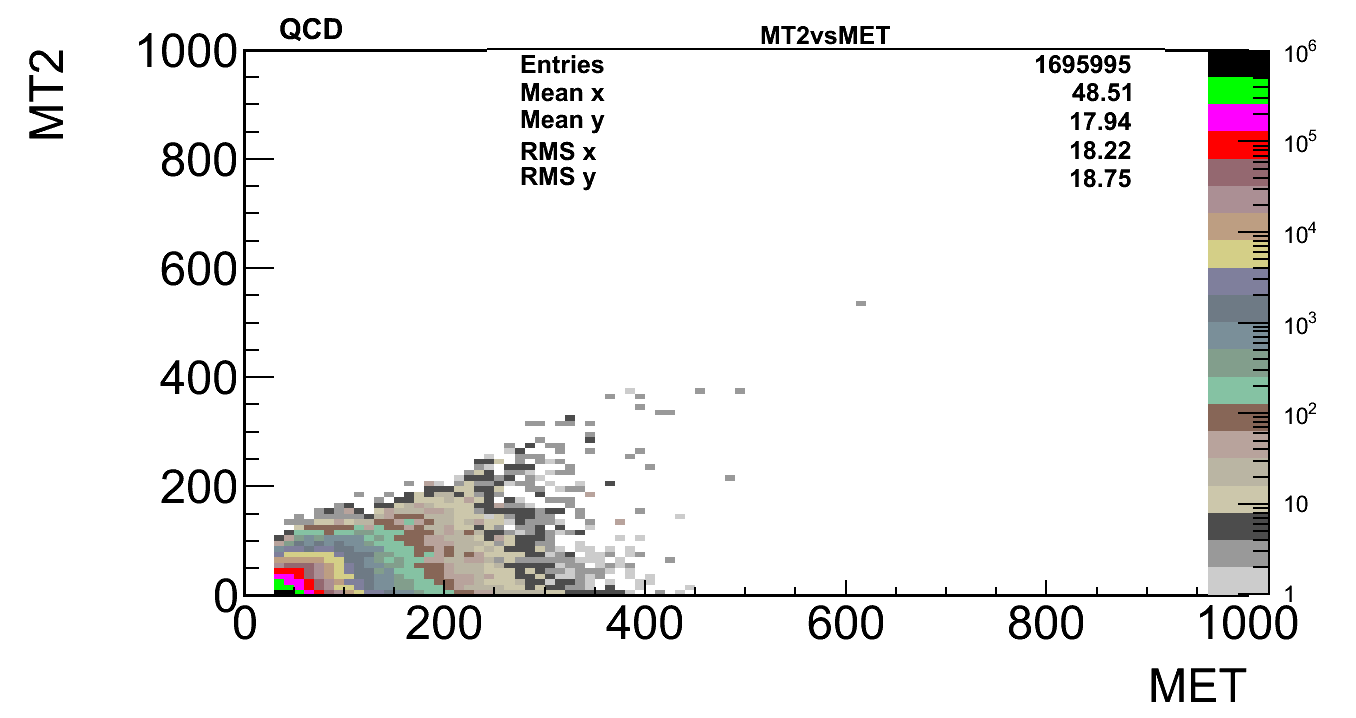
\includegraphics[angle=00,width=0.5\textwidth]{figs/MT2-MET-before-AllCuts-QCD.png}&
%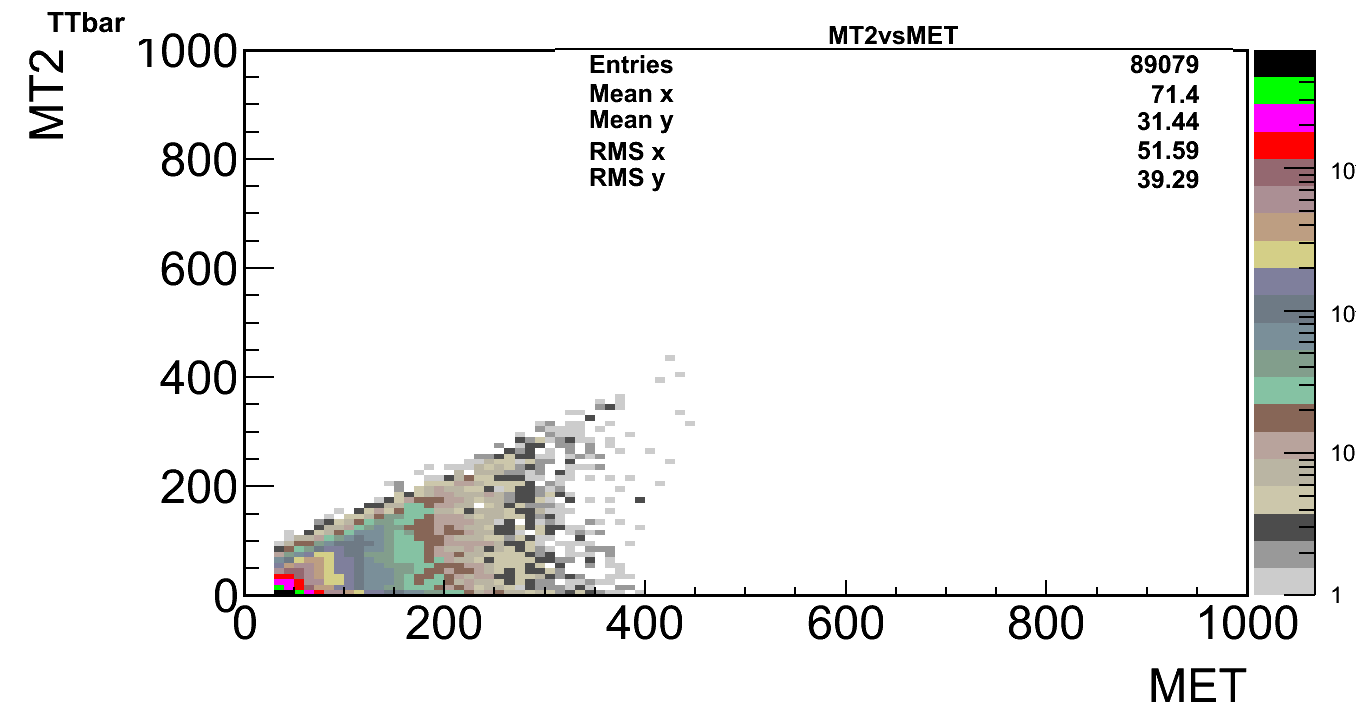
\includegraphics[angle=00,width=0.5\textwidth]{figs/MT2-MET-before-AllCuts-Top.png}\\
%	\mbox{\small{(a).data sample}} & \mbox{\small{(b).QCD sample}} & \mbox{\small{(c).top sample}}\\
%\end{array}$
%\end{center}
%\caption{Scatter plot of \met and \mttwo}
%\label{fig:MT2METCorr}
%\end{figure}

To figure out the effects of pile-up reweighting, it was plotted the number of vertices before and after pile-up reweighting which as it is seen , this reweighting corrects MC as expected. 

\begin{figure}[!Hhtb]
\begin{center}$
\begin{array}{cc} 
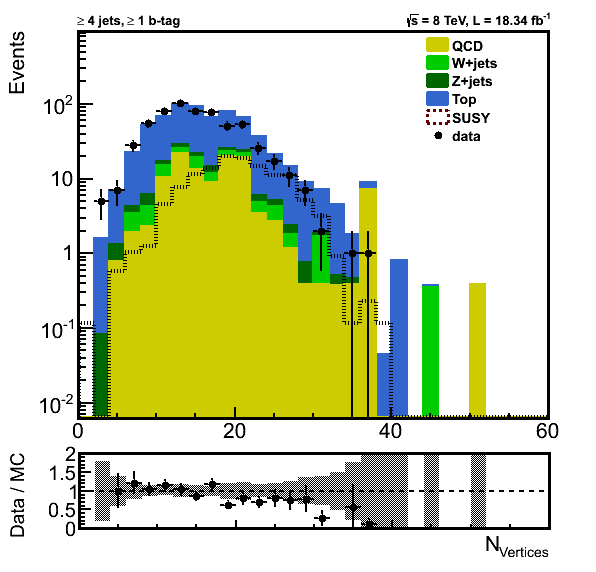
\includegraphics[angle=00,width=0.5\textwidth]{figs/NVert-NoPU.png}&
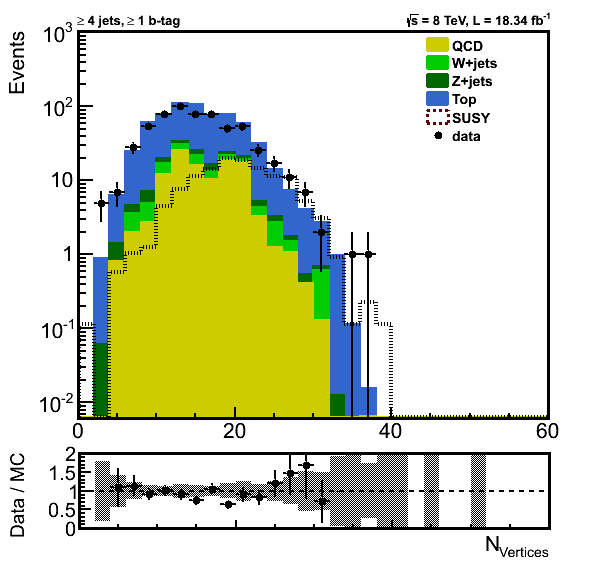
\includegraphics[angle=00,width=0.5\textwidth]{figs/NVert-WithPU.png}\\
	\mbox{\small{(a)}} & \mbox{\small{(b)}} \\
\end{array}$
\end{center}
\caption{Distribution of number of vertices for data before(a) and after (b) pile-up reweighting}
\label{fig:NVerticesPileUpData}
\end{figure}

%\begin{figure}[!Hhtb]
%\begin{center}$
%\begin{array}{ccc} 
%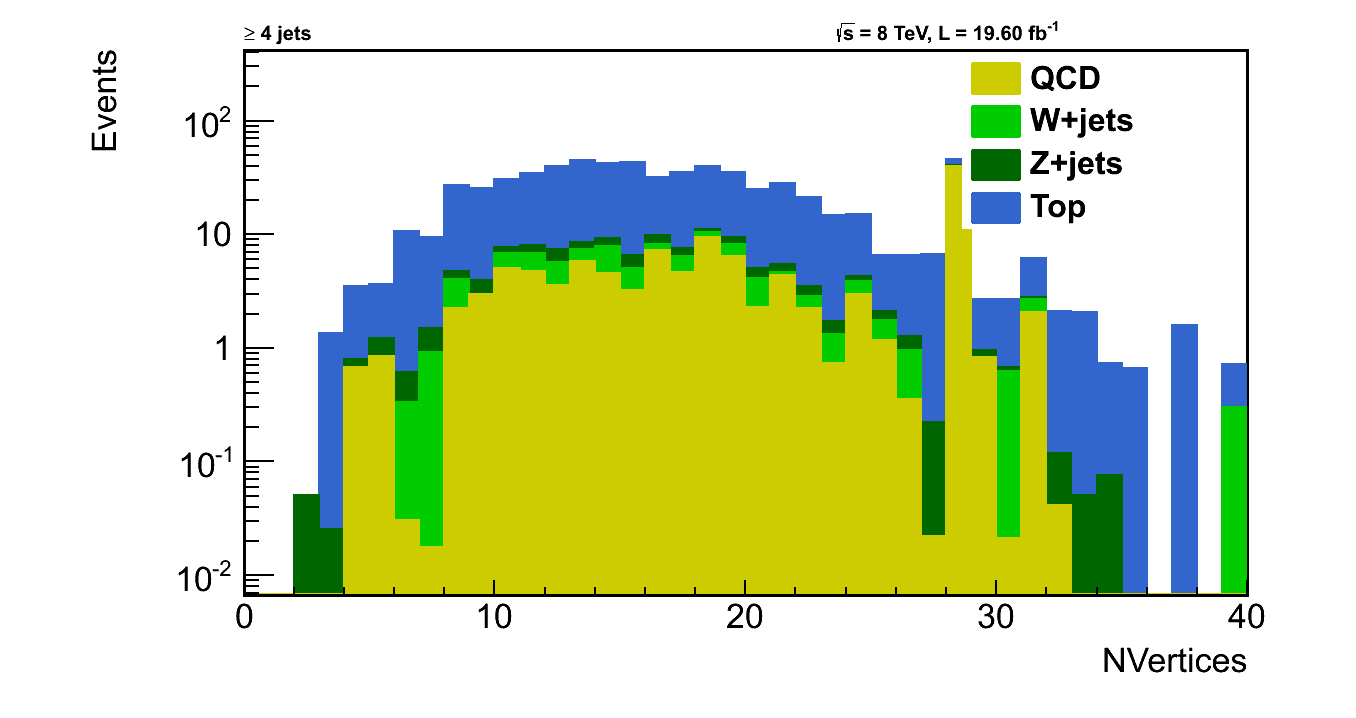
\includegraphics[angle=00,width=0.5\textwidth]{figs/NVertices-MC-NoPU-NoRatio.png}&
%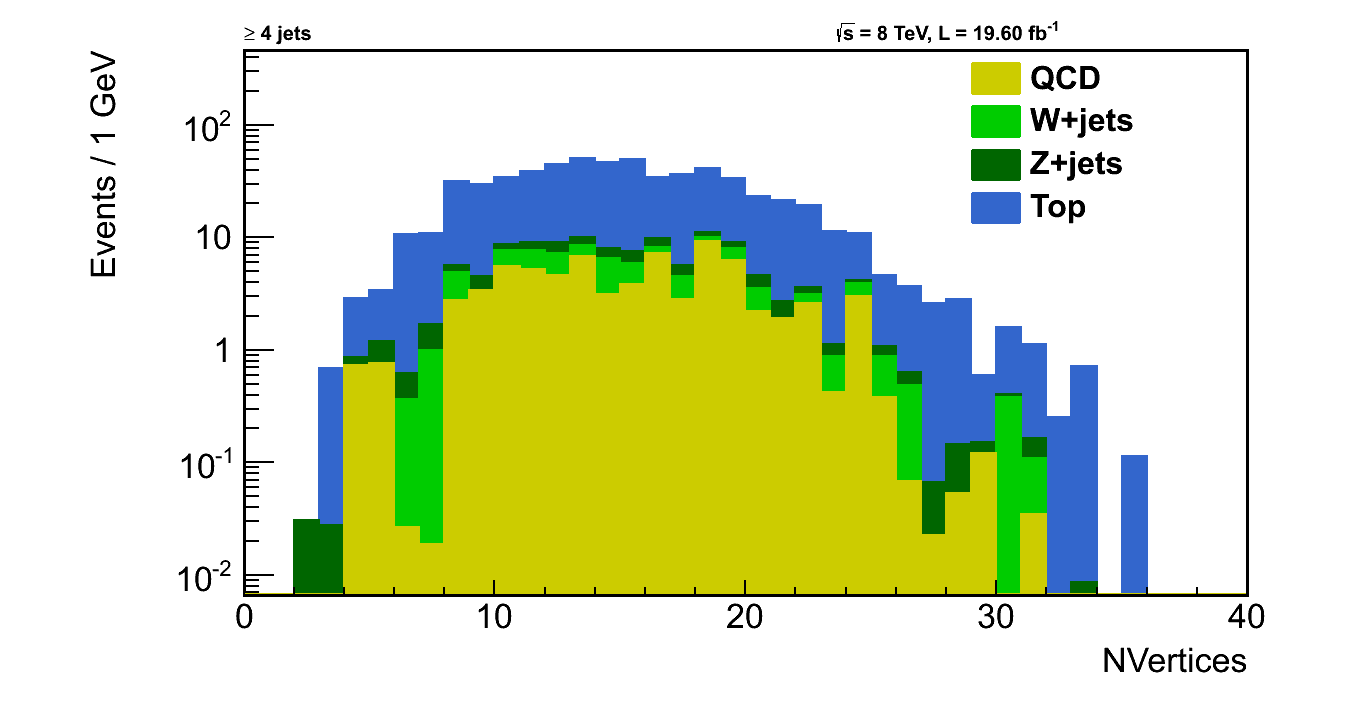
\includegraphics[angle=00,width=0.5\textwidth]{figs/NVertices-MC-PU-NoRatio.png}\\
%	\mbox{\small{(a)}} & \mbox{\small{(b)}} \\
%\end{array}$
%\end{center}
%\caption{Distribution of number of vertices for MC before(a) and after(b) pile-up reweighting }
%\label{fig:NVerticesPileUpMC}

%\end{figure}
